\chapter{Objekt-Semantik}

\subsubsection*{Klassendiagramm (Struktur)}
... beschreibt den Aufbau und das Zusammenspiel von Klassen innerhalb des Systems. Meist auf Basis von Dingen.

\begin{figure}[hbt]
  \centering
  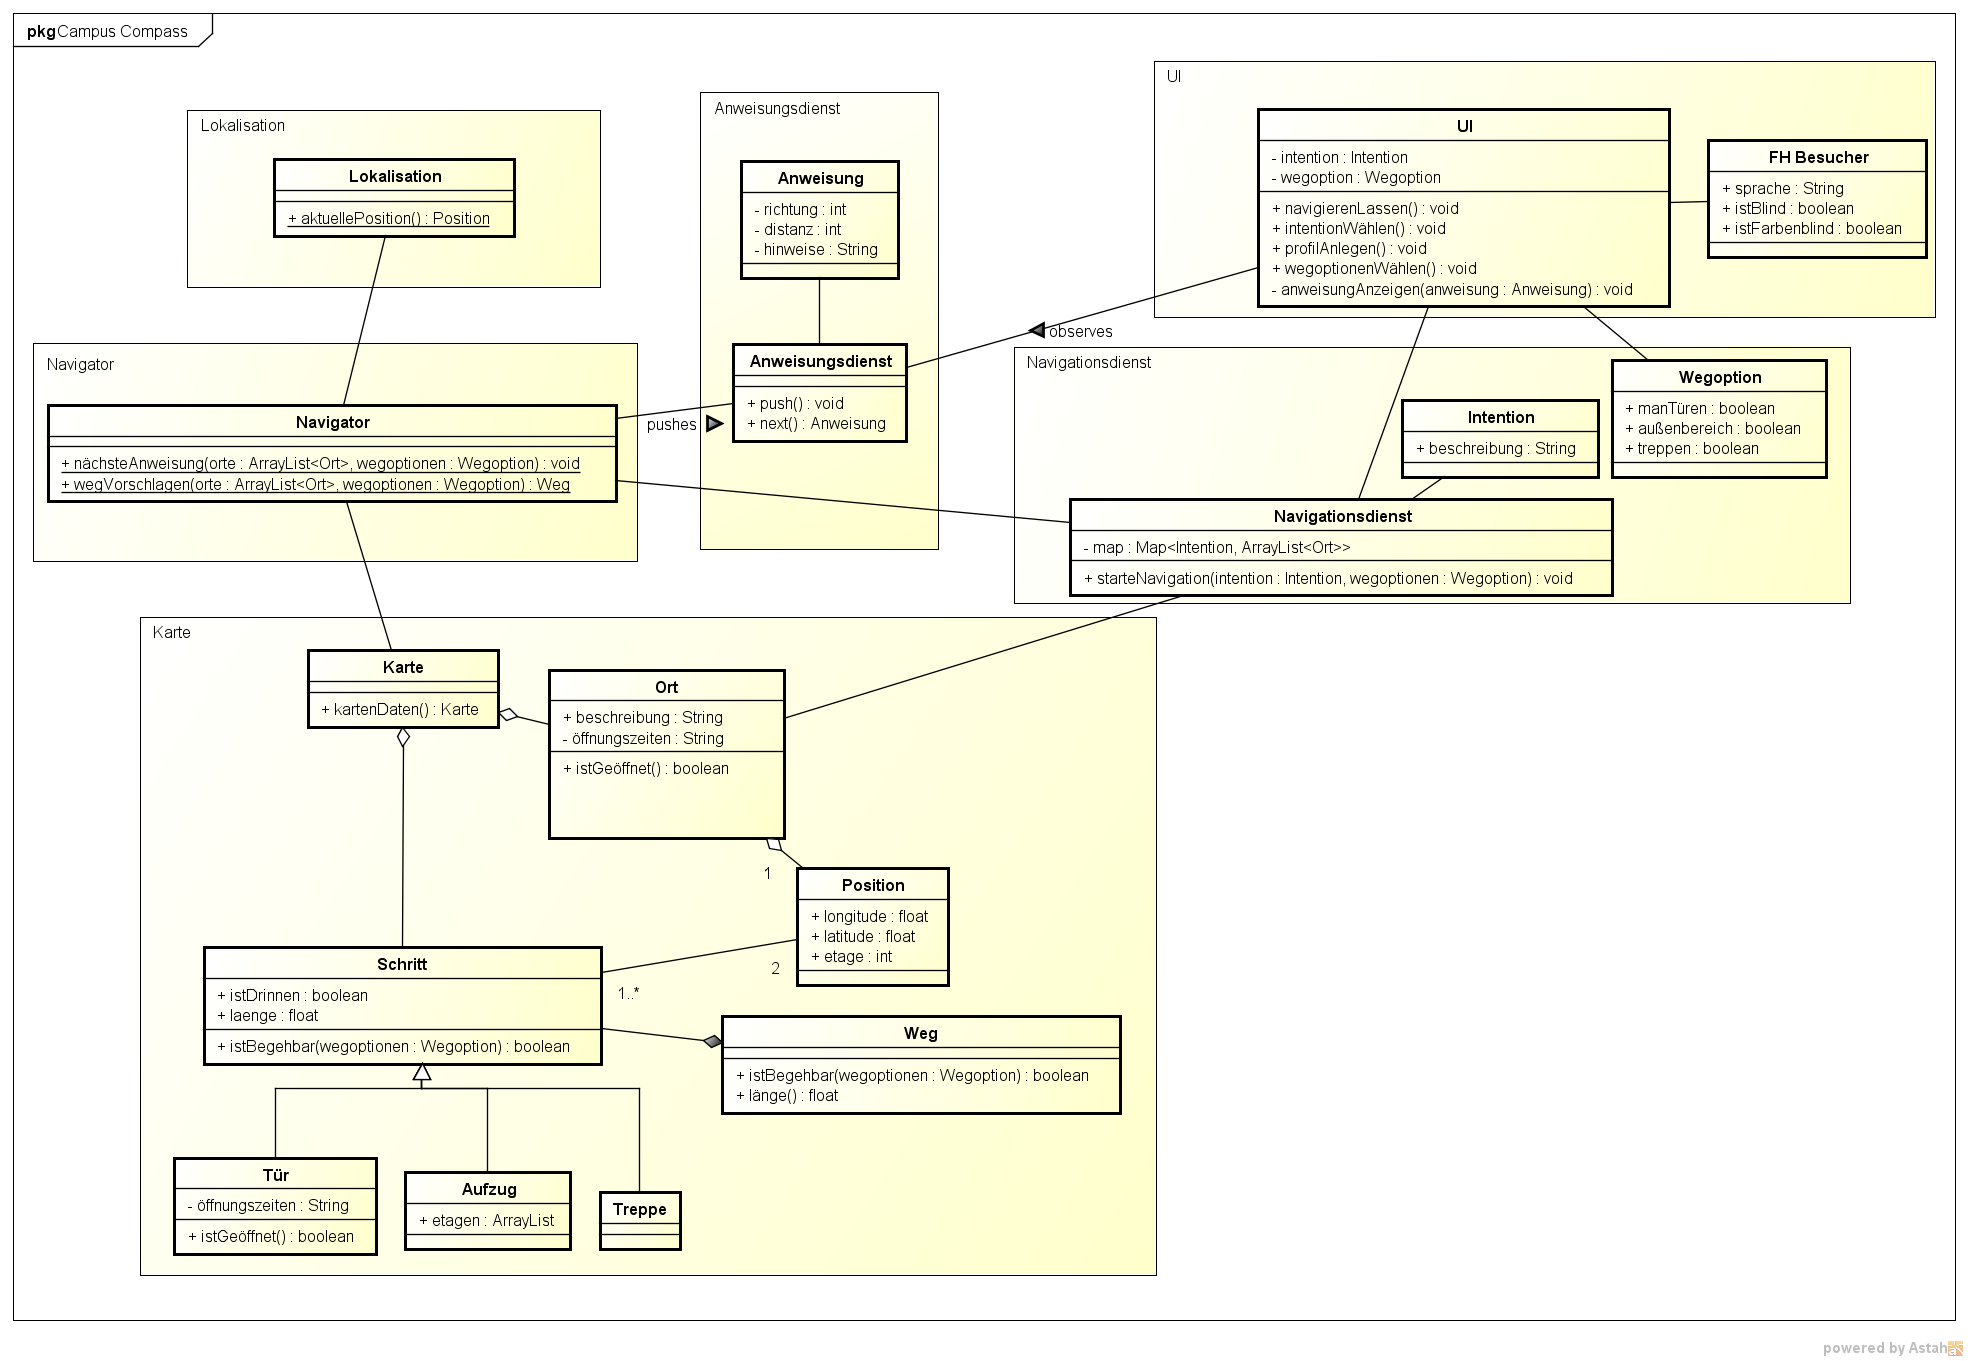
\includegraphics[width=\linewidth]{img/klassendiagramm.png}
  \label{img:klassendiagramm}
  \caption{Klassendiagramm}
\end{figure}

\subsubsection*{Zustandsdiagramm (Verhalten)}
... zeigt den Zustand eines Obejkts zur Laufzeit.

\begin{figure}[hbt]
  \centering
  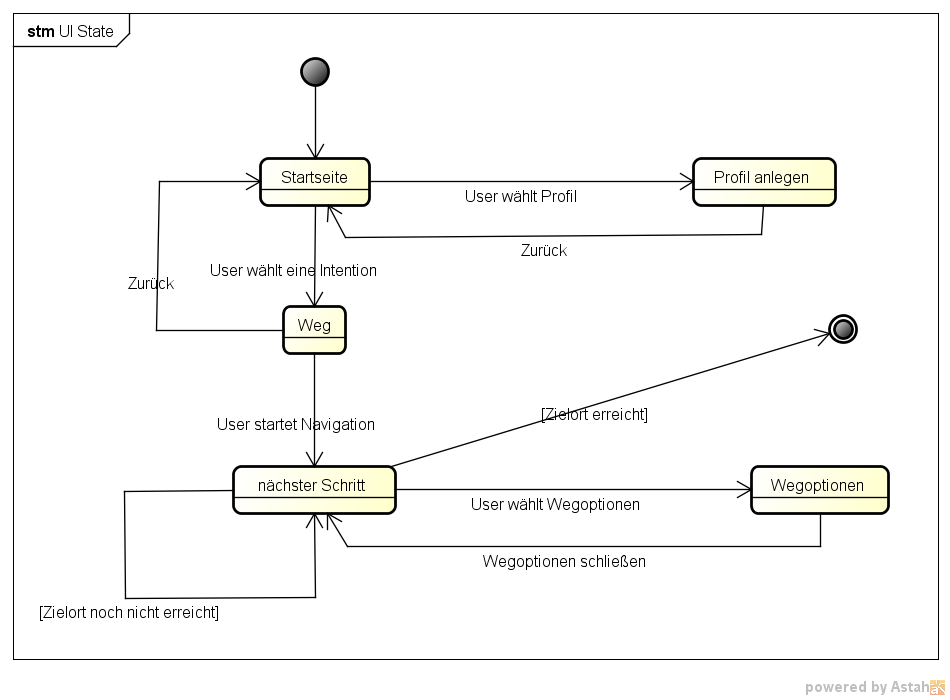
\includegraphics[width=\linewidth]{img/zustandsdiagramm.png}
  \label{img:zustandsdiagramm}
  \caption{Zustandsdiagramm}
\end{figure}

\subsubsection*{Sequenzdiagramm (Verhalten)}
... beschreibt die Interaktion (Kommunikation) von Objekten/Komponenten im zeitlichen Verlauf in einer bestimmten Szene.

\begin{figure}[hbt]
  \centering
  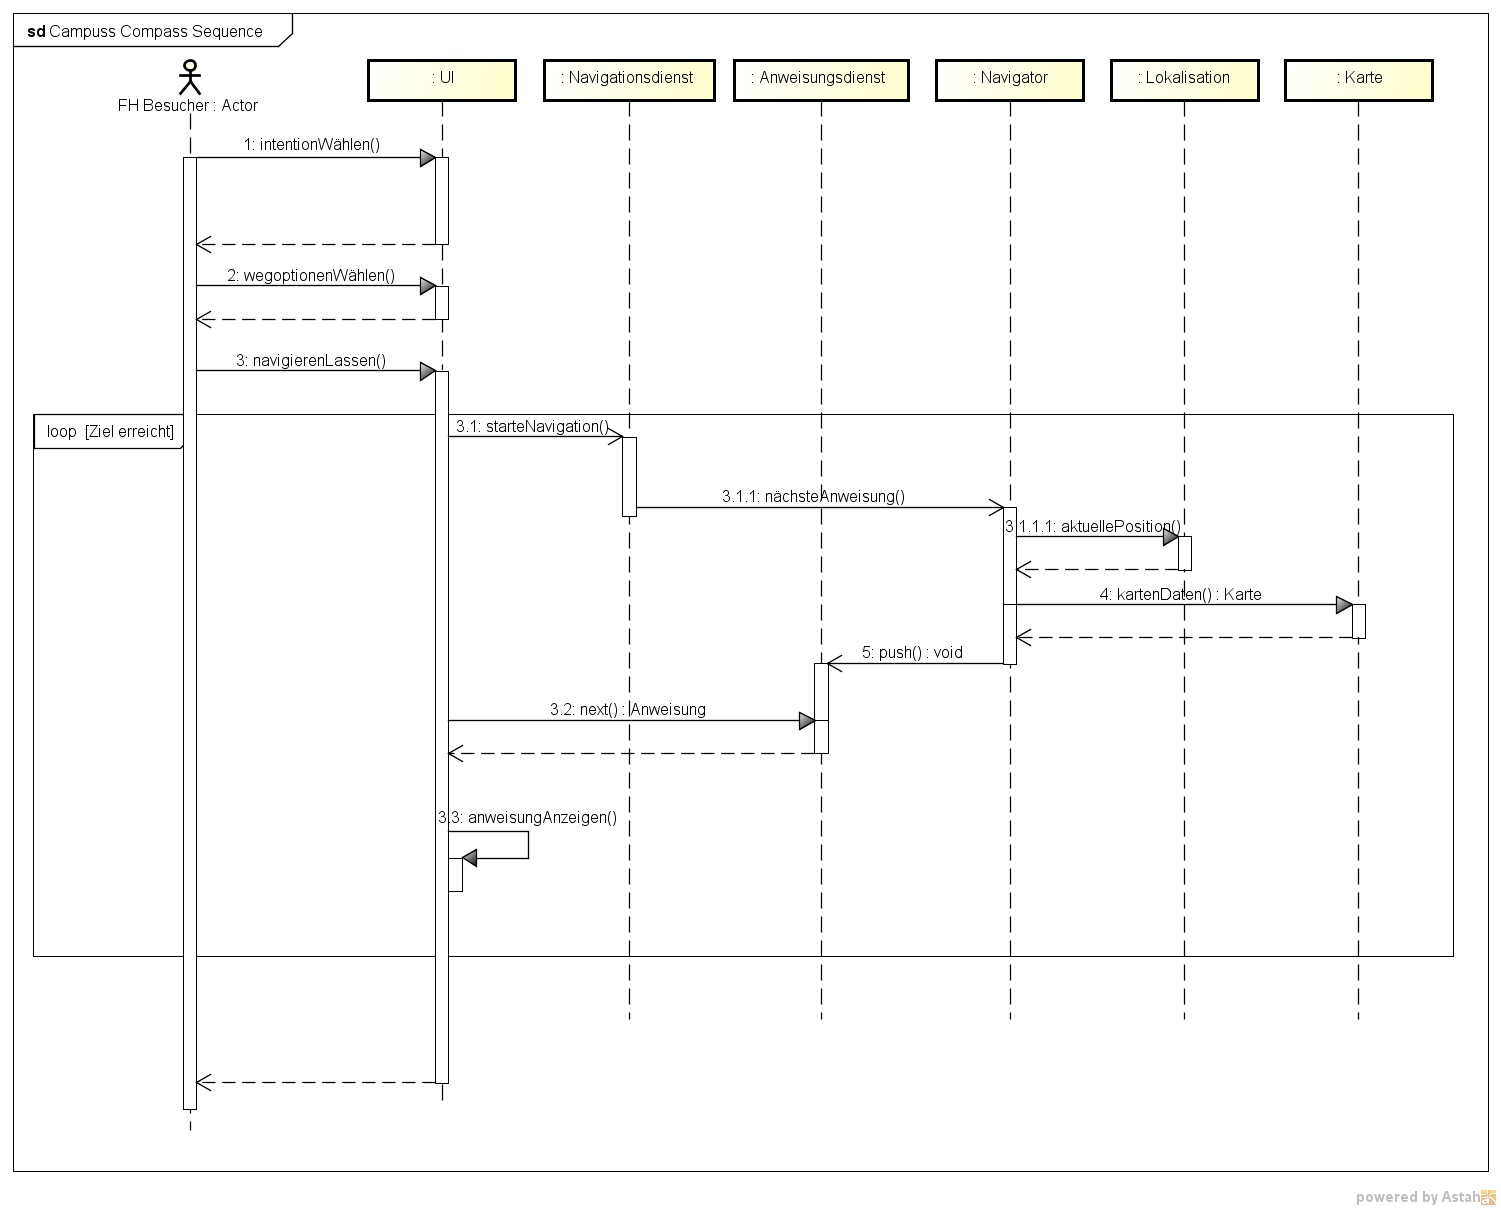
\includegraphics[width=\linewidth]{img/sequenzdiagramm.png}
  \label{img:sequenzdiagramm}
  \caption{Sequenzdiagramm}
\end{figure}